\chapter{Testing and Evaluation} \label{t-e}

\section{Introduction} \label{t-e--introduction}

Chapters \ref{a-d} and \ref{s-i} described the design and implementation of a progressive web application for use in a home-brewing context. In this chapter, the testing method is discusses with results in section \ref{t-e--testing}. The next chapter evaluates the implementation as a whole in section \ref{t-e--evaluation}. This is followed by a review of the requirements, both functional and non-functional, in section \ref{t-e--requirements-review}.

\section{Testing} \label{t-e--testing}

The testing framework used was mocha and complemented by the `chai' and `sinon' packages. This meant simple and targeted tests could be created. \cite{mocha}

Using a headless browser such as PhantomJS means tests can be run automatically in a browser environment without having to open a browser such as Chrome or FireFox. \cite{phantomjs}

To run the tests created with mocha in PhantomJS a test runner called Karma was used. \cite{karma} This also handled processing the files through the same Webpack config that is used to build the site normally.

The tests created are for testing basic rendering of the Preact components and also that certain elements do not render if not authenticated. Figure \ref{figure-tests} shows tests running in a terminal environment. \footnote{Note if ESLint passes linting, it usually doesn't output anything but for this screenshot the `debug' flag has been added}

\begin{figure}[H]
  \centering
    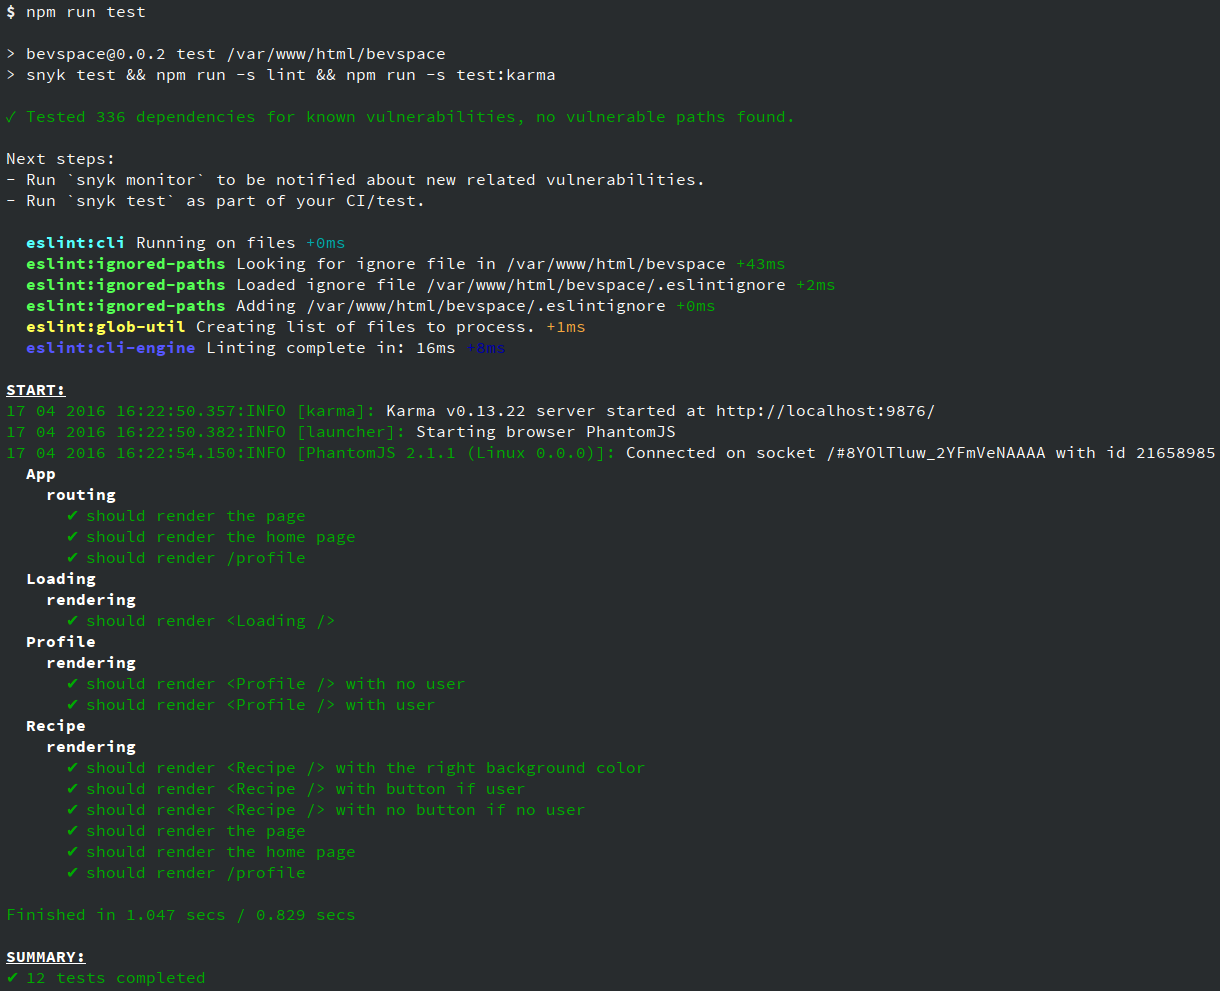
\includegraphics[width=\textwidth,height=\textheight,keepaspectratio]{tests}
  \caption{Output to the terminal when running `npm run test'}
  \label{figure-tests}
\end{figure}

For the continuous integration, the tests running include Snyk, linting and the previously mentioned rendering tests. \ref{a-d--continuous-integration}

\section{Evaluation} \label{t-e--evaluation}

This testing in the previous section \ref{t-e--testing} shows stability in the application and the foundations for a maintainable testing setup. This section will evaluate the implementation.

The project since the PID (project initiation document, see appendix \ref{appendix:pid}) has changed dramatically. Due to the initial client moving away from the project a change in focus occurred from from home-brewing to performance. % add ref to appendix

Overall, where the project is weakened is through the planning and structuring. With more discipline this project could have fulfilled more of the initial requirements. Using a traditional project management approach such as using Gantt charts could have helped here. Trello was not used in favour of GitHub issues. With a larger team Trello and the kanban structure would have been useful for higher-level planning.

Saying this, a lot of the technologies used in the project are in their infancy, as seen in section \ref{s-i--interesting-problems}. This means potentially the work flow, tools and technologies will all be outdated soon and replaced with better iterations.

People and their needs don't change so much. Performance will always be important. So the research and work done in this area was very beneficial. Principles such as offline first powered by service worker caching and clientside databases as implemented in this artefact look to be the future of the web industry.

While there is testing for the application itself, user testing should have been done in order to evaluate the research reviewing in section \ref{l-r--perceived-performance}. This could be included in any future work on the artefact.

\section{Requirements Review} \label{t-e--requirements-review}

This section reviews the requirements set in the artefact design (see section \ref{a-d--requirements}), each requirement is reintroduced with discussion as to how successful each requirement was met.

\subsection{Functional Requirements} \label{t-e--requirements--functional}

This section will review the functional requirements.

\subsubsection{Finding recipes}

\begin{itemize}
  \item As a \textbf{user}, I want to \textbf{browse for recipes}

  This is fulfilled with a list of recipes (as seen in Figure \ref{figure-implementation-screenshots}) simply showing the name of the brew, the author fo the brew and the colour of the brew as a strip on the left for context. There is also the IBU (International Bittering Unit) and ABV (Alcohol by Volume) displayed to the right.

  One problem found, when rendering close to 1000 recipes into the DOM there is significant lag. Looking into the cause of this jank it was found that there was a large amount of garbage collection. Using pagination or a virtual list would solve this problem.

\end{itemize}

\subsubsection{Starting a brew}

\begin{itemize}
  \item As a \textbf{user}, I want to \textbf{select and start a brew from any recipe}

  When selecting a recipe there is a button to start the brew. This adds the recipe to the brews section but doesn't start any timers. This allows for the brews to be in `staging` area. This functionality could be clearer as currently seen as starting the brew.
\end{itemize}

\subsubsection{Managing a brew}

\begin{itemize}
  \item As a \textbf{user}, I want to \textbf{be shown what point I am in a brew}

  When a brew has started (as shown in Figure \ref{figure-implementation-screenshots}) there is a progress circle with a percentage and completed tasks in the brewing timeline are coloured green to indicate they have been completed.

  For future work this could be extended to have a `current' task which knows how long a task should take for better context. Also push notifications could be implemented for each task another great use for a service worker. Unfortunately due to needing to use Google Cloud Messaging a Node.js server would be needed to be handle this, complicating the application. \cite{google_cloud_messaging}

  \item As a \textbf{user}, I want to \textbf{add notes to key stages of a brew}

  This functionality wasn't fulfilled in the current implementation, but with CouchDB (and similarly PouchDB) not needing schemas, arbitrary data can be added to documents. Therefore this functionality, with more time would be easily implemented.

  \item As a \textbf{user}, I want to \textbf{review and evaluate the brew on completion}

  As with the previous functionality this wasn't fulfilled and would be fairly simple to implement.
\end{itemize}

\subsection{Non-Functional Requirements} \label{t-e--requirements--non-functional}

This section will review the non-functional requirements.

\begin{itemize}
  \item \textbf{Compliant to WCAG 2 level AAA to ensure enough contrast ``when viewed by someone having color deficits or when viewed on a black and white screen". \cite{colour_contrast}}

    When looking at the example of the items on the page, there was some need to improve the contrast.

    Fortunately using SASS (as chosen in section \ref{a-d--t--styling}) this is achieved very easily by changing variables. For example, \verb|color: \$brown;| producing \verb|\#943938| to \verb|color: darken(\$brown, 10\%);| producing \verb|\#6F2B2A|.

    Table \ref{table-contrast-changes} shows how the new darkened version of the brown colour is WCAG 2 AAA compliant.

    \begin{table}[H]
    \centering
    \begin{tabular}{|l|l|l|l|}
    \hline
    \textbf{Colour} & \textbf{Contrast Ratio} & \textbf{WCAG 2 AA Compliant} & \textbf{WCAG 2 AAA Compliant} \\ \hline
    \cellcolor[HTML]{943938}{\color[HTML]{FFFFFF} \textbf{\#943938}} & 6.24 & Yes & No                       \\ \hline
    \cellcolor[HTML]{6F2B2A}{\color[HTML]{FFFFFF} \textbf{\#6F2B2A}} & 8.81 & Yes & Yes                      \\ \hline
    \end{tabular}
    \caption{Showing the compliance of the different colours against the background}
    \label{table-contrast-changes}
    \end{table}

  \item \textbf{Be documented so that others can maintain}

    For future maintaining of the project documentation should be used. The README file shows instructions to build and work with the project. Comments throughout components give explanation for code that isn't straight forward.

    A package called commitizen was used to enforce the contributing guidelines for project. \cite{commitizen}

  \item \textbf{Conform to the performance budget that is set in initial development}

    From the budget set in section \ref{table-performance-budget}, here are the results with the implemented site show in table \ref{table-performance-budget-results}.

    Notice how times change before and after caching with the service worker.

    \begin{table}[H]
    \centering
    \begin{tabular}{|l|l|l|l|}
    \hline
    \textbf{Site}        & \textbf{Start Render} & \textbf{Document Complete} & \textbf{Fully Loaded} \\ \hline
    Malt.to              & 2.190s                & 3.998s                     & 4.145s                \\ \hline
    Proposed solution    & 1.752s                & 3.198s                     & 3.316s                \\ \hline
    Implementation       & 1.086s                & 2.118s                     & 3.914s                \\ \hline
    Implementation w/ SW & 0.890s                & 1.784s	                    & 4.895s	              \\ \hline
    \end{tabular}
    \caption{Performance budget calculation with results}
    \label{table-performance-budget-results}
    \end{table}

    As shown the performance budget at the current state of the implementation was succeeded. This would be tracked for future work.

  \item \textbf{Pass tests generated throughout and running through continuous integration (such as Travis CI)}

    As described in detail in section \ref{t-e--testing}, the artefact is passing all tests including Snyk, Linting and Karma. However, by the nature of Snyk looking for vulnerabilities constantly without maintenance these tests could fail.

\end{itemize}

\section{Testing and Evaluation Summary} \label{t-e--testing-and-evaluation-summary}

This chapter introduced the testing and some evaluation of the implementation. In section \ref{t-e--testing} testing locally and with Travis CI is explained. This was followed by an evaluation of the implementation in section \ref{t-e--requirements-review}.
